\documentclass[a4paper,12pt]{article}

% Process graphics.
\usepackage{graphicx}
% Create clickable links in the pdf
\usepackage[bookmarks=true,pdfborder={0 0 0}]{hyperref}

\usepackage{csquotes}
% Format links
\usepackage{url}

\usepackage[style=ieee]{biblatex}
\addbibresource{auxil/referencias.bib}

% Keep floats in their sections
\usepackage[section]{placeins}
% List code in the lstlisting environment
\usepackage{listings}
% Options for the lstlisting environment
\lstset{numbers=left, showspaces=false, showstringspaces=false, frame=single}
% Format tables with some special features (e.g. auto-width columns)
% \usepackage{tabulary}

%%%%% LEGACY LaTeX (pdflatex) - USE XeLaTeX IF AVAILABLE (SEE BELOW) %%%%%%%%%%
% Set the font to sans-serif
\renewcommand{\familydefault}{\sfdefault}
%%%%% ENABLE IF XeLaTeX or LuaLaTeX IS AVAILABLE FOR BEST RESULTS %%%%%%%%%%%%%
% Enables doing changes in the font.
% \usepackage{fontspec}
% Set the font. [Requires fontspec] If you don't have CMU Bright you can use another one, e.g. Arial.
% \setmainfont[Mapping=tex-text]{CMU Bright}
%%%%%%%%%%%%%%%%%%%%%%%%%%%%%%%%%%%%%%%%%%%%%%%%%%%%%%%%%%%%%%%%%%%%%%%%%%%%%%%

% Enables setting cutom colors
\usepackage{xcolor}
\usepackage{sectsty}
\definecolor{blue1}{RGB}{52, 90, 138}
\definecolor{blue2}{RGB}{79, 129, 189}
\sectionfont{\color{blue1}}
\subsectionfont{\color{blue2}}
\subsubsectionfont{\color{blue2}}

\usepackage[spanish]{babel}
\usepackage{amsmath}
\usepackage{appendix}
\usepackage{graphicx}
\usepackage{graphicx}

% --- Personalización de nombres para figuras y tablas en español ---
\renewcommand{\figurename}{Figura}
\renewcommand{\figureautorefname}{Figura}
\renewcommand{\tablename}{Tabla}
\renewcommand{\tableautorefname}{Tabla}

% Set the color of the Table of Contents header to black
\renewcommand{\contentsname}{\textcolor{black}{Table of Contents}}
% Set the title formatting
\makeatletter
\renewcommand{\maketitle}{\bgroup\setlength{\parindent}{0pt}
    \begin{flushleft}
    {\Huge\textbf{\@title}}
    \end{flushleft}\egroup
}
\makeatother


% Typeset keystrokes
% \usepackage{keystroke}

%%%%%%%%%%%%%%%%%%%%%%%%%%%%%%%%%%%%%%%%%%%%%%%%%%%%%%%%%%%%%%%%%%%%%%%%%%%%%%%%

\AtBeginEnvironment{tikzpicture}{\shorthandoff{:!<>|}}
\begin{document}

    % Set and insert the title.
    \title{Documento de diseño del sistema\\}
    \maketitle


    \section*{\color{black}Sentido del documento}

    Este documento describe el diseño del sistema de software para este proyecto.
    Se propondrán soluciones para los problemas de diseño y se describirán las decisiones de diseño tomadas.
    El documento de diseño del sistema (SDD) es un documento de referencia para el diseño del sistema de software y la arquitectura del software.
    Es un documento vinculante para el desarrollo del software y la implementación de los subsistemas.

    El contenido de este documento sigue y se ajusta a los requisitos especificados en el IEEE 1016--1998\autocite{IEEE1016-1998}


    % Set the Table of Contents depth and inert the ToC.
    \setcounter{tocdepth}{2}
    \tableofcontents


    \section{Introducción}\label{sec:introduccion}
    Este documento describe el diseño del sistema de software para el proyecto BiciFast.
    El diseño del sistema se basa en los requisitos funcionales y no funcionales especificados en el documento de requisitos del sistema (SRD).\autocite{SRD-BiciFast}
    Este documento está destinado a ser utilizado por los desarrolladores del sistema, los arquitectos de software y los diseñadores de la interfaz de usuario.

    \subsection{Propósito del documento}\label{subsec:proposito-del-documento}
    El propósito de este documento es proporcionar una descripción detallada del diseño del sistema de software para el proyecto BiciFast.

    \subsection{Definiciones, acrónimos y abreviaturas}\label{subsec:definiciones-acronimos-y-abreviaturas}


    \phantomsection

    \addcontentsline{toc}{section}{Referencias}


    \printbibliography


    \section{Objetivos de diseño}\label{sec:objetivos-de-diseno}
    Para diseñar este sistema, se ha priorizado:
    \begin{enumerate}
        \item \textbf{Modularidad:} Hacer que las partes del sistema sean independientes entre ellas, permitiendo la fácil modificación de los módulos.
        \item \textbf{Simplicidad:} Hacer que el sistema sea fácil de entender y de usar.
        \item \textbf{Separación de responsabilidades:} Separar las diferentes partes del sistema en módulos independientes, cada uno con su propia responsabilidad.
        \item \textbf{Escalabilidad:} Hacer que el sistema sea fácil de escalar y de modificar en el futuro.
    \end{enumerate}


    \section{Composición del sistema, arquitectura y capas}\label{sec:composicion-del-sistema-arquitectura-y-capas}
    \input{composición-del-sistema,-arquitectura-y-capas}

    \section{Diseño de la Interfaz Gráfica de Usuario (GUI)}\label{sec:diseno-de-la-interfaz-grafica-de-usuario-(gui)}
        La interfaz gráfica de la aplicación está desarrollada empleando Java Swing, orientada a un uso intuitivo por parte de los usuarios finales.
    La aplicación permitirá el acceso a los servicios de alquiler de bicicletas a través de una serie de pantallas conectadas por un flujo lógico y sencillo.
    Por falta de tiempo, sólo se ha realizado el diseño de las pantallas relativas al usuario, dejando de lado las pantallas de administración y mantenimiento de estaciones y bicicletas.
    Esta sección será actualizada en futuras versiones del documento para incluir las pantallas restantes.

    \subsection{Resumen de las Pantallas}\label{subsec:resumen-de-las-pantallas}

    A continuación se detallan las principales pantallas de la aplicación:

    \subsubsection{Pantalla 1: Iniciar sesión}
    \begin{itemize}
        \item \textbf{Nombre:} DiaLogin
        \item \textbf{Objetivo:} Permitir al usuario autenticarse en el sistema.
        \item \textbf{Componentes:}
        \begin{itemize}
            \item Campo de texto para correo electrónico.
            \item Campo de texto para contraseña.
            \item Botón ``Iniciar sesión''.
            \item Enlace para registrarse si no se tiene cuenta.
        \end{itemize}
        \item \textbf{Flujo:} Al iniciar sesión con éxito, se redirige a la pantalla principal.
    \end{itemize}

    \subsubsection{Pantalla 2: Principal del usuario}
    \begin{itemize}
        \item \textbf{Nombre:} VPrincipalUsuario
        \item \textbf{Objetivo:} Servir como punto central de acceso a las funciones principales.
        \item \textbf{Componentes:}
        \begin{itemize}
            \item Vista de mapa con la localización de las estaciones.
            \item Botones para ver estaciones, alquilar, devolver bicicleta.
            \item Acceso al perfil del usuario.
        \end{itemize}
        \item \textbf{Flujo:} Permite navegar hacia la selección de estación o a la edición del perfil.
    \end{itemize}

    \subsubsection{Pantalla 3: Bicicletas en una estación}
    \begin{itemize}
        \item \textbf{Nombre:} DiaBicis
        \item \textbf{Objetivo:} Mostrar bicicletas disponibles en una estación concreta.
        \item \textbf{Componentes:}
        \begin{itemize}
            \item Lista de bicicletas con identificador, tipo y estado.
            \item Botón de reserva/alquiler.
        \end{itemize}
    \end{itemize}

    \subsubsection{Pantalla 4: Perfil de usuario}
    \begin{itemize}
        \item \textbf{Nombre:} DiaUsuario
        \item \textbf{Objetivo:} Permitir la visualización y edición de los datos personales.
        \item \textbf{Componentes:}
        \begin{itemize}
            \item Nombre, correo electrónico, idioma preferido.
            \item Historial de alquileres.
            \item Botón ``Editar perfil''.
        \end{itemize}
    \end{itemize}

    \subsubsection{Pantalla 5: Selección de idioma}
    \begin{itemize}
        \item \textbf{Nombre:} VIdioma
        \item \textbf{Objetivo:} Configurar el idioma de la aplicación.
        \item \textbf{Componentes:}
        \begin{itemize}
            \item Lista desplegable de idiomas.
            \item Botón ``Guardar''.
        \end{itemize}
    \end{itemize}

    \subsection{Estilo visual y usabilidad}

    La interfaz presenta un diseño sencillo, funcional y adaptado a usuarios con diferentes niveles de experiencia tecnológica. Los colores son neutros y consistentes, y los componentes están dispuestos de manera que facilitan la navegación. Los textos son breves y claros, y los botones tienen etiquetas intuitivas.

    \subsection{Diagrama de navegación}\label{subsec:diagrama-de-navegacion}
    El diagrama de navegación muestra cómo se conectan las diferentes pantallas de la aplicación y cómo los usuarios pueden navegar entre ellas. Cada pantalla está conectada a las demás según el flujo lógico del uso de la aplicación, permitiendo un acceso fácil a todas las funcionalidades.
    \begin{figure}[h!]
        \centering
        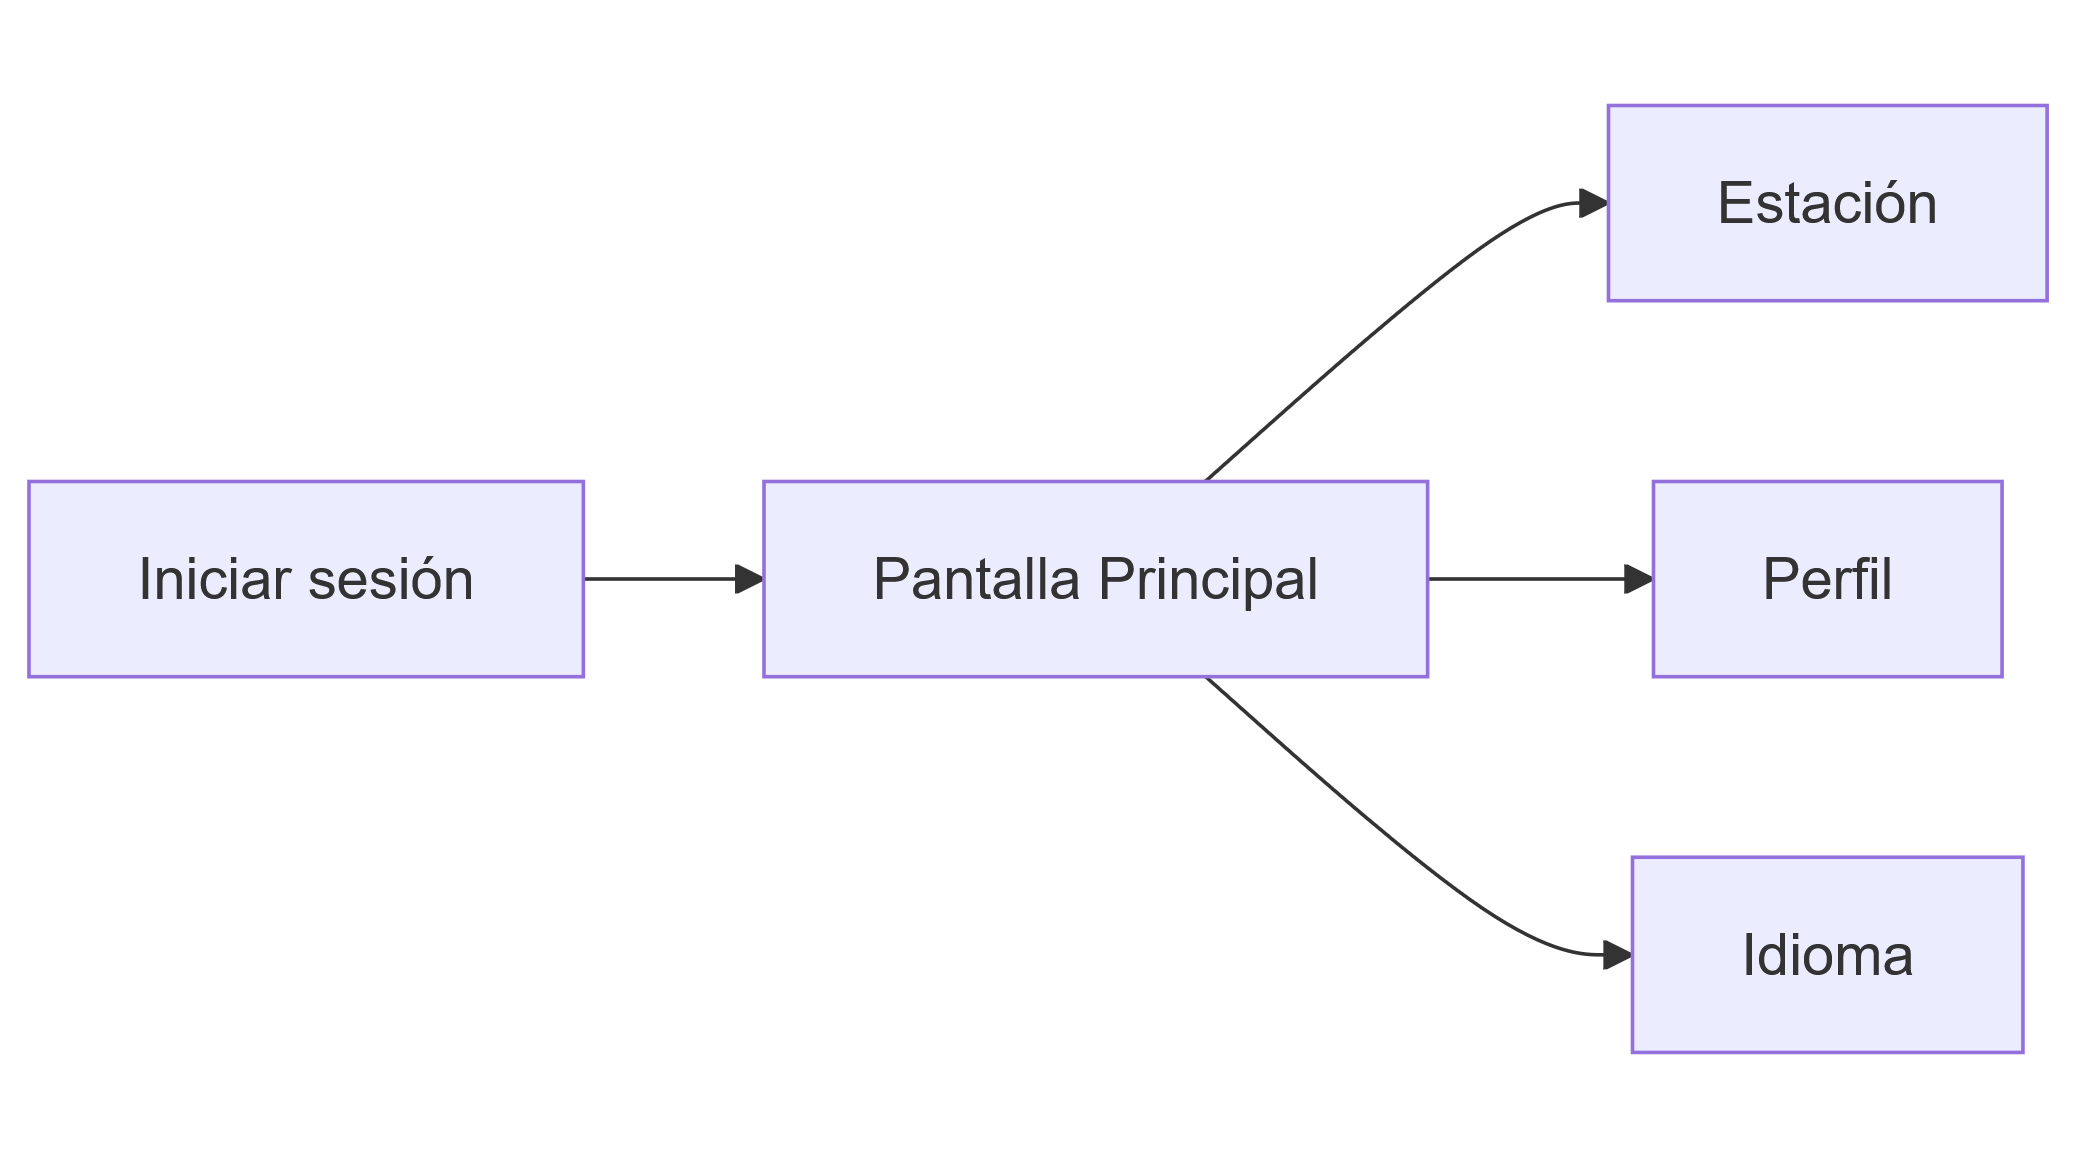
\includegraphics[width=0.7\textwidth]{imagenes/diagrama_navegacion.png}
        \caption{Diagrama de navegación de la aplicación}
        \label{fig:diagrama_navegacion}
    \end{figure}

    \clearpage

    \subsection{Bocetos}\label{subsec:mockups}

    A continuación se presentan los mockups de las pantallas principales de la aplicación.
    Estos mockups ilustran el diseño visual y la disposición de los elementos en cada pantalla.
    Estas han sido creadas con la herramienta Draw.io y se encuentran en formato PNG para su inclusión en el documento. %todo: cita aquí
    \begin{figure}[ht]
        \centering
        \includegraphics{imagenes/bicifast - p1 - Iniciar sesión.drawio}
        \caption{Pantalla 1 - Iniciar sesión}
        \label{fig:bicifast---p1---iniciar-sesion.drawio}
    \end{figure}

    \begin{figure}
        \centering
        \includegraphics[scale=0.50]{imagenes/bicifast - pantalla 2 -principal usuario}
        \caption{Pantalla 2 - Principal del usuario}
        \label{fig:bicifast---pantalla-2--principal-usuario}
    \end{figure}

    \begin{figure}
        \centering
        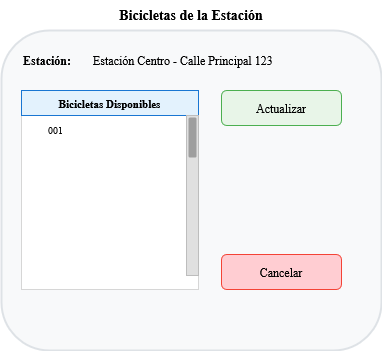
\includegraphics{imagenes/bicifast - pantalla 3 -bicicletas en una estacion.drawio}
        \caption{Pantalla 3 - Bicicletas en una estación}
        \label{fig:bicifast---pantalla-3--bicicletas-en-una-estacion.drawio}
    \end{figure}

    \begin{figure}
        \centering
        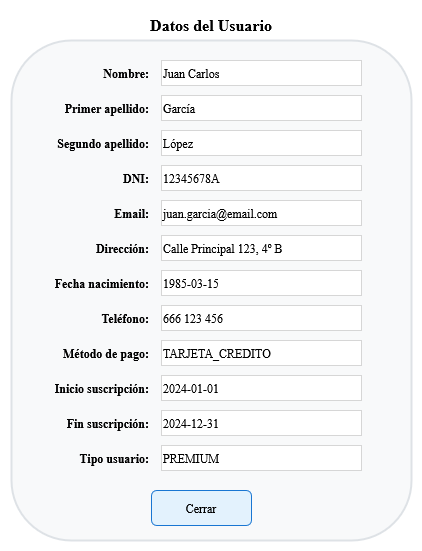
\includegraphics{imagenes/bicifast - pantalla 4 -datos del usuario.drawio}
        \caption{Pantalla 4 - Datos del usuario}
        \label{fig:bicifast---pantalla-4--datos-del-usuario.drawio}
    \end{figure}

    \begin{figure}
        \centering
        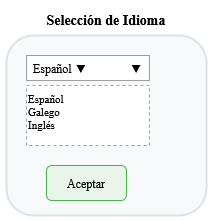
\includegraphics{imagenes/bicifast - pantalla 5 -Seleccion de idiomadrawio}
        \caption{Pantalla 5 - Selección de idioma}
        \label{fig:bicifast---pantalla-5--seleccion-de-idiomadrawio}
    \end{figure}
%    \begin{figure}[H]
%        \centering
%        \includegraphics[width=0.6\textwidth]{ruta/a/bicifast - p1 - Iniciar sesión.drawio.png}
%        \caption{Pantalla 1 - Iniciar sesión}
%    \end{figure}
%
%    \begin{figure}[H]
%        \centering
%        \includegraphics[width=0.6\textwidth]{ruta/a/bicifast - pantalla 2 -principal usuario.png}
%        \caption{Pantalla 2 - Principal del usuario}
%    \end{figure}
%
%    \section{Hardware/software mapping}
%    % Content: This section describes how the subsystems are mapped onto existing hardware and software components. A UML deployment diagram accompanies the description. The existing components are often off-the-shelf components. If the components are distributed on different nodes, the network infrastructure and the protocols are also described.
%    % NOTE: You may find a figure snippet at the end of this document.
%
%
%    \section{Persistent data management} % Optional
%    % Content: This section describes how the entity objects are mapped to persistent storage. It contains a rationale of the selected storage scheme, file system or database, a description of the selected database and database administration issues.
%
%
%    \section{Access control and security} % Optional
%    % Content: This section describes the access control and security issues based on the nonfunctional requirements in the requirements analysis document. It also describes the implementation of the access matrix based on capabilities or access control lists, the selection of authentication mechanisms and the use of encryption algorithms.
%
%
%    \section{Global software control} % Optional
%    % Content: This section describes the control flow of the system, in particular, whether a monolithic, event-driven control flow or concurrent processes have been selected, how requests are initiated and specific synchronization issues.
%
%
%    \section{Boundary conditions} % Optional
%    % Content: This section describes the use cases how to start up the separate components of the system, how to shut them down, and what to do if a component or the system fails.
%

\end{document}

